\documentclass[conference]{IEEEtran}
\usepackage{cite}
\usepackage{amsmath,amssymb}
\usepackage{graphicx}
\usepackage{booktabs}
\usepackage{algorithm}
\usepackage{algpseudocode}

\graphicspath{{figures/}}

\begin{document}

\title{Sequential Causal Training of Windowed PINNs for The  Lorenz ODE System}

% \author{
% \IEEEauthorblockN{Ikramul Hasan Moral, Md. Abu Bakar, Samiur Rahman Omlan,\\
% Md. Touhidul Islam, Fariha Islam, and Muhammad Nomani Kabir}
% \IEEEauthorblockA{Department of Computer Science and Engineering, United International University, Dhaka, Bangladesh\\
% imoral223489@bscse.uiu.ac.bd, mbakar223200@bscse.uiu.ac.bd, somlan223195@bscse.uiu.ac.bd,\\
% mislam223435@bscse.uiu.ac.bd, fislam223431@bscse.uiu.ac.bd, kabir@cse.uiu.ac.bd}
% }


\author{\IEEEauthorblockN{Ikramul Hasan Moral}
\IEEEauthorblockA{\textit{Computer Science And Engineering} \\
imoral223489@bscse.uiu.ac.bd\\
0112230489}\\

\and
\IEEEauthorblockN{Md. Abu Bakar}
\IEEEauthorblockA{\textit{Computer Science And Engineering} \\
mbakar223200@bscse.uiu.ac.bd\\
0112230200}
\and
\IEEEauthorblockN{Samiur Rahman Omlan}
\IEEEauthorblockA{\textit{Computer Science And Engineering} \\
somlan223195@bscse.uiu.ac.bd\\
0112230195}
\and
\IEEEauthorblockN{Md. Touhidul Islam}
\IEEEauthorblockA{\textit{Computer Science And Engineering} \\
mislam223435@bscse.uiu.ac.bd \\0112230435}
\and
\IEEEauthorblockN{Fariha Islam}
\IEEEauthorblockA{\textit{Computer Science And Engineering} \\
fislam223431@bscse.uiu.ac.bd \\ 0112230431}
\and
\IEEEauthorblockN{Dr. Muhammad Nomani Kabir}
\IEEEauthorblockA{\textit{Professor, Dept of CSE} \\
\textit{United International University}\\
kabir@cse.uiu.ac.bd}
}


\maketitle

\begin{abstract}
We study a physics-informed neural network (PINN) approximation of a single full-cycle orbit of the Lorenz three-state system on $t\in[0,13.26446]$. We trained a single network on the full interval that produce a combined state root-mean-square error (RMSE) of 2.237. To address this long horizon problem, we divide the interval in total 27 windows. Each window has a separate network and an initial state that is fixed to the predicted endpoint of the previous window. In each window, Adam reduces the residual in four stages. In each stage, we use causal weights and causal weighted loss to reduce the loss of all earlier points. Then, L-BFGS minimizes the loss using the unweighted residual mean. A numerical reference is used to monitor the training but is not used for optimization or stopping. We reported, in a single-seed run the windowed model gives a combined RMSE of $6.97\times10^{-5}$ on 13,265 evaluation times and a dense-grid residual mean square of $1.87\times10^{-7}$.  The full-interval and windowed runs also vary in terms of number of parameters, sampling and optimizer schedule. In contrast, these are described with the word configurations, not isolation of the effect of causal weighting.

\end{abstract}

\begin{IEEEkeywords}
physics-informed neural network, Lorenz system, causal training, time windows, ordinary differential equation, windowed PINN
\end{IEEEkeywords}

\section{Introduction}
The Lorenz-system model is a three-state, nonlinear ordinary differential equation (ODE) that was obtained from a reduced flow model \cite{lorenz1960}. It has an initial-value problem which provides a simple test of the convergence of a learned continuous-time function from a specified trajectory over a long interval. A reference trajectory is provided by numerical integration. A PINN is trained with the residual of the ODE instead of the solution samples \cite{raissi2019}. To train a a long horizon problem using traditional PINN is not suggested by previous works\cite{wang2024causal}. It couples early and late times, but the state at a later time is determined by the previous trajectory. To overcome this ordering, Wang \emph{et al.} suggested the use of time-dependent residual weights PINN training \cite{wang2024causal}. An initial condition can also be met by construction using a hard trial solution  \cite{lagaris1998}. We use both concepts, we split the time period in equal 27 windows and a separate network for every windows. The initial state is fixed with the endpoint predicted in one window of the next. The parameters of a trained window is copied to the next trainable window. This paper provides an implementation and its saved results. An interval that completes a full-cycle loop for the chosen initial state is $[0,13.26446]$. We report one implementation and its saved result on $[0, 13.26446]$ which is essentially an closed orbit. The actual training goal and window handoff is then given and compared to a saved single-network training of the same initial-value problem. The state error, ODE residual, causal weights residual are also checked. The comparison is descriptive because multiple configuration options are changing simultaneously.



\section{Problem and Background}
In this section we introduce the mathematical goal of our study and place our configuration within the framework of existing neural-network techniques. We first describe the exact equations and the initial value problem of the Lorenz trajectory that we want the model to learn. Then we explain the existing methods that we used and then we merged them.

\subsection{Lorenz Equations}
Our main object is a three-state nonlinear ordinary differential equation (ODE) that we need to solve. The Lorenz system general form \cite{matthews2024pinnde} is:

\begin{equation}
\begin{aligned}
\frac{dx}{dt}
  &= \kappa\ell
     \left(\frac{1}{\kappa^2+\ell^2}
           -\frac{1}{\kappa^2}\right)yz,\\
\frac{dy}{dt}
  &= \kappa\ell
     \left(\frac{1}{\ell^2}
           -\frac{1}{\kappa^2+\ell^2}\right)xz,\\
\frac{dz}{dt}
  &= \frac{\kappa\ell}{2}
     \left(\frac{1}{\kappa^2}
           -\frac{1}{\ell^2}\right)xy.
\end{aligned}
\label{eq:lorenz1960}
\end{equation}

Suppose the state vector is given by $u=[x,y,z]^\mathsf{T}$. 


% Physical wavenumbers: \kappa and \ell.
% Window index: k.

\[
\begin{aligned}
\kappa&=2,\quad \ell=1,\\
a_x&=2(1/5-1/4)=-1/10=-0.1,\\
a_y&=2(1-1/5)=8/5=1.6,\\
a_z&=(2/2)(1/4-1)=-3/4=-0.75.
\end{aligned}
\]

\begin{equation}
\dot{x}=-0.1\,yz,\qquad \dot{y}=1.6\,xz,\qquad \dot{z}=-0.75\,xy,
\label{eq:ode}
\end{equation}


\[
\begin{gathered}
u=[x,y,z]^\mathsf{T}\in\mathbb{R}^{3},\\
a=[a_x,a_y,a_z]^\mathsf{T}=[-0.1,1.6,-0.75]^\mathsf{T},\\
\frac{du}{dt}=f(u),\qquad f:\mathbb{R}^{3}\to\mathbb{R}^{3},\\
f(u)=\begin{bmatrix}a_x\,yz\\a_y\,xz\\a_z\,xy\end{bmatrix}
=\begin{bmatrix}-0.1\,yz\\1.6\,xz\\-0.75\,xy\end{bmatrix}.
\end{gathered}
\]






For our experiment we used the coefficients $a=[a_x,a_y,a_z]^\mathsf{T}=[-0.1,1.6,-0.75]^\mathsf{T}$. We track the system starting from an initial state \cite{matthews2024pinnde} of $u(0)=[0.5,0.75,1.0]^\mathsf{T}$ until a final time of $T=13.26446$. On this particular rounded endpoint, the reference trajectory nearly returns to its starting state. It is very similar but not exactly closed so we call this interval a nearly closed orbit and not an exact period.


\subsection{Related Work}
In this study we are making an experimental investigation of a series of well known concepts. The approach adopted is a PINN that embeds the physics residual into the training objective \cite{raissi2019}. We use a hard trial-function design \cite{lagaris1998} to ensure our starting state precisely at the point we want to implement it . Learning long trajectories is a well-known challenge due to the ordering of the time axis so we take inspiration from the causal residual weighting technique \cite{wang2024causal}. Lastly segmenting the timeline is based on ideas of causal sweeping and temporal decomposition \cite{penwarden2023}. Our implementation is an investigation of the performance of the individual components in this particular closed orbit of lorenz system.

\section{Windowed PINN}
This section explains the implementation of windowed PINN with causal weigths. This section also contains the model construction, physics enforcement, window segmentation, its handoff and the sequence in how the optimizer works for this particular case. 
\subsection{Network Structure}
We used several modelling strategies to approximate the solution for Lorenz system trajectory over  $[0,T]$, where $T=13.26446$ is one closed loop for the chosen initial state. We first tried one network to learn the entire trajectory at once. As it failed by stucking in a platue so we tried to split the time interval in equal segments.

\begin{figure}[t]
\centering
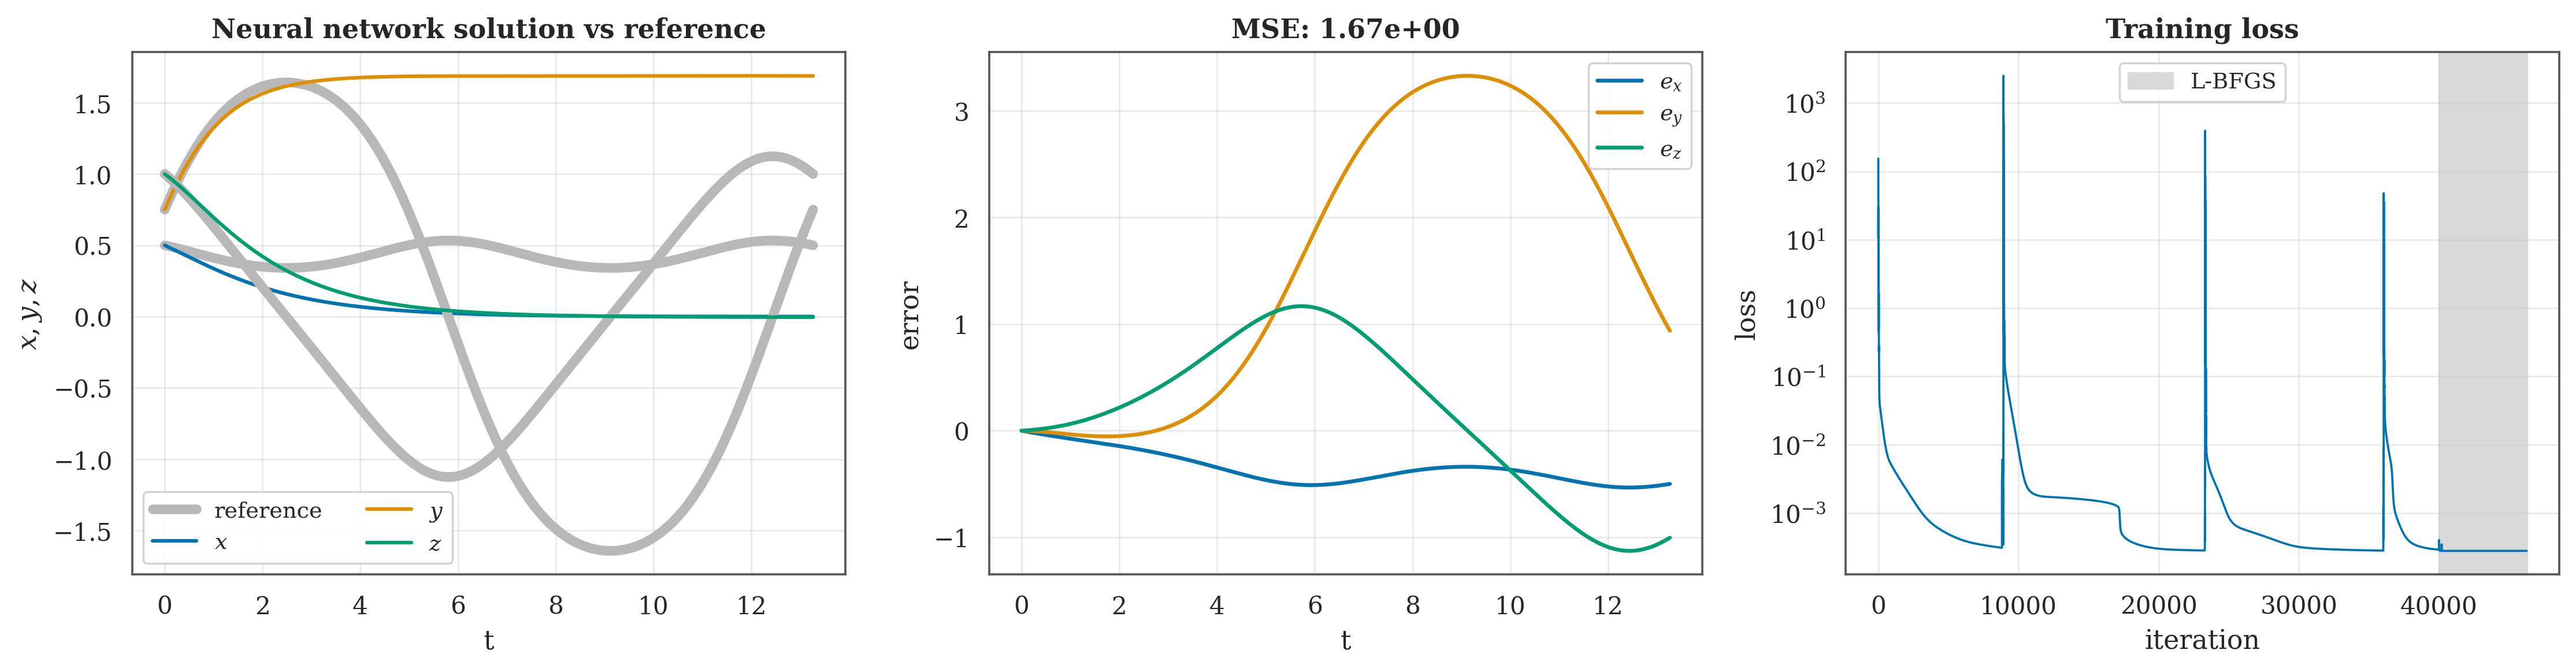
\includegraphics[width=\columnwidth]{figures/platue-results.png}
\caption{Training result of a single network , entire time at once}
\label{fig:plateau}
\end{figure}

We tried to keep the split window closer to 0.5, as small windows are better \cite{wang2024causal}. In first experiment, we used one network with 27 segmented time period to train the model sequentially. We noticed that, whenever the window is moved to the new one, the previous learning is lost or degraded. This results in significant increase in loss with RMSE of 2.237. To address these issues, we introduced WPINN (Windowed PINN). We split the total time $[0,T]$ equally into 27 windows and gave each window its own network.


\[
\begin{aligned}
t_k&=kT/27,\qquad k=0,\ldots,27,\\
W_k&=[t_k,t_{k+1}],\qquad k=0,\ldots,26,\\
\Delta t&=T/27\approx0.4912763,\\
N_k(\,\cdot\,;\theta_k)&:W_k\to\mathbb{R}^{3}.
\end{aligned}
\]


Each aprroximately $0.491$ time units wide. Shorter window gives each network an easier piece to learn, therefore we tried to keep the window size closer to 0.5. 

Each window has its own network  $N_k(t;\theta_k)$ with 1 input layer (t), 4 hidden layers of 60 neurons with tanh unit, and with an output layer with 3 output $(x,y,z)$. 

\[
\begin{aligned}
P_{\mathrm{window}}&=120+3(3660)+183=11{,}283,\\
P_{\mathrm{total}}&=27P_{\mathrm{window}}=304{,}641.
\end{aligned}
\]

For the model parameter initialization we used xavier-uniform weights and zero biases. The 27 networks don't share parameters but the windows has shared boundary. The completed windows predicted endpoint for the boundary is used for the initial state of the next window. 

\subsection{Window Handoff}
As Lorenz system is an initial value problem, we enforce the initial state of each window through a trial solution.

\begin{equation}
\begin{aligned}
\hat{u}_k(t)
  &=u_{0,k}+(t-t_k)N_k(t;\theta_k),\\
&\qquad t\in W_k,\quad k=0,\ldots,26.
\end{aligned}
\label{eq:trial}
\end{equation}


\[
\begin{gathered}
u_{0,k},N_k(t;\theta_k),\hat{u}_k(t)\in\mathbb{R}^{3},\quad t-t_k\in\mathbb{R},\\
\hat{u}_k(t_k)=u_{0,k}+0\,N_k(t_k;\theta_k)=u_{0,k},\\
u_{0,0}=[0.5,0.75,1.0]^\mathsf{T}.
\end{gathered}
\]


where $k=0,\ldots,26$, $t_k$ is the starting time of window $k$, and $u_{0,k}$
is its fixed starting state. At $t=t_k$, the second term is zero, so
$\hat{u}_k(t_k)=u_{0,k}$ regardless of the network parameters
\cite{lagaris1998}. The first window uses the trial initial state, every later windows uses the predicted value of the last window as its initial state.

\begin{equation}
u_{0,k+1}=\hat{u}_k(t_{k+1}), \qquad k=0,\ldots,25.
\label{eq:handoff}
\end{equation}

\[
\hat{u}_{k+1}(t_{k+1})=u_{0,k+1}=\hat{u}_k(t_{k+1}).
\]

$\theta_{k+1}\leftarrow\theta_k, \qquad k=0,\ldots,25$, here window k+1 starts from a copy of the weights of window k then train on its own parameters . This makes the predicted values continuous at the window boundaries. As the starting point of the later windows is predicted, it can carry error from earlier windows. 

\begin{figure}[t]
\centering
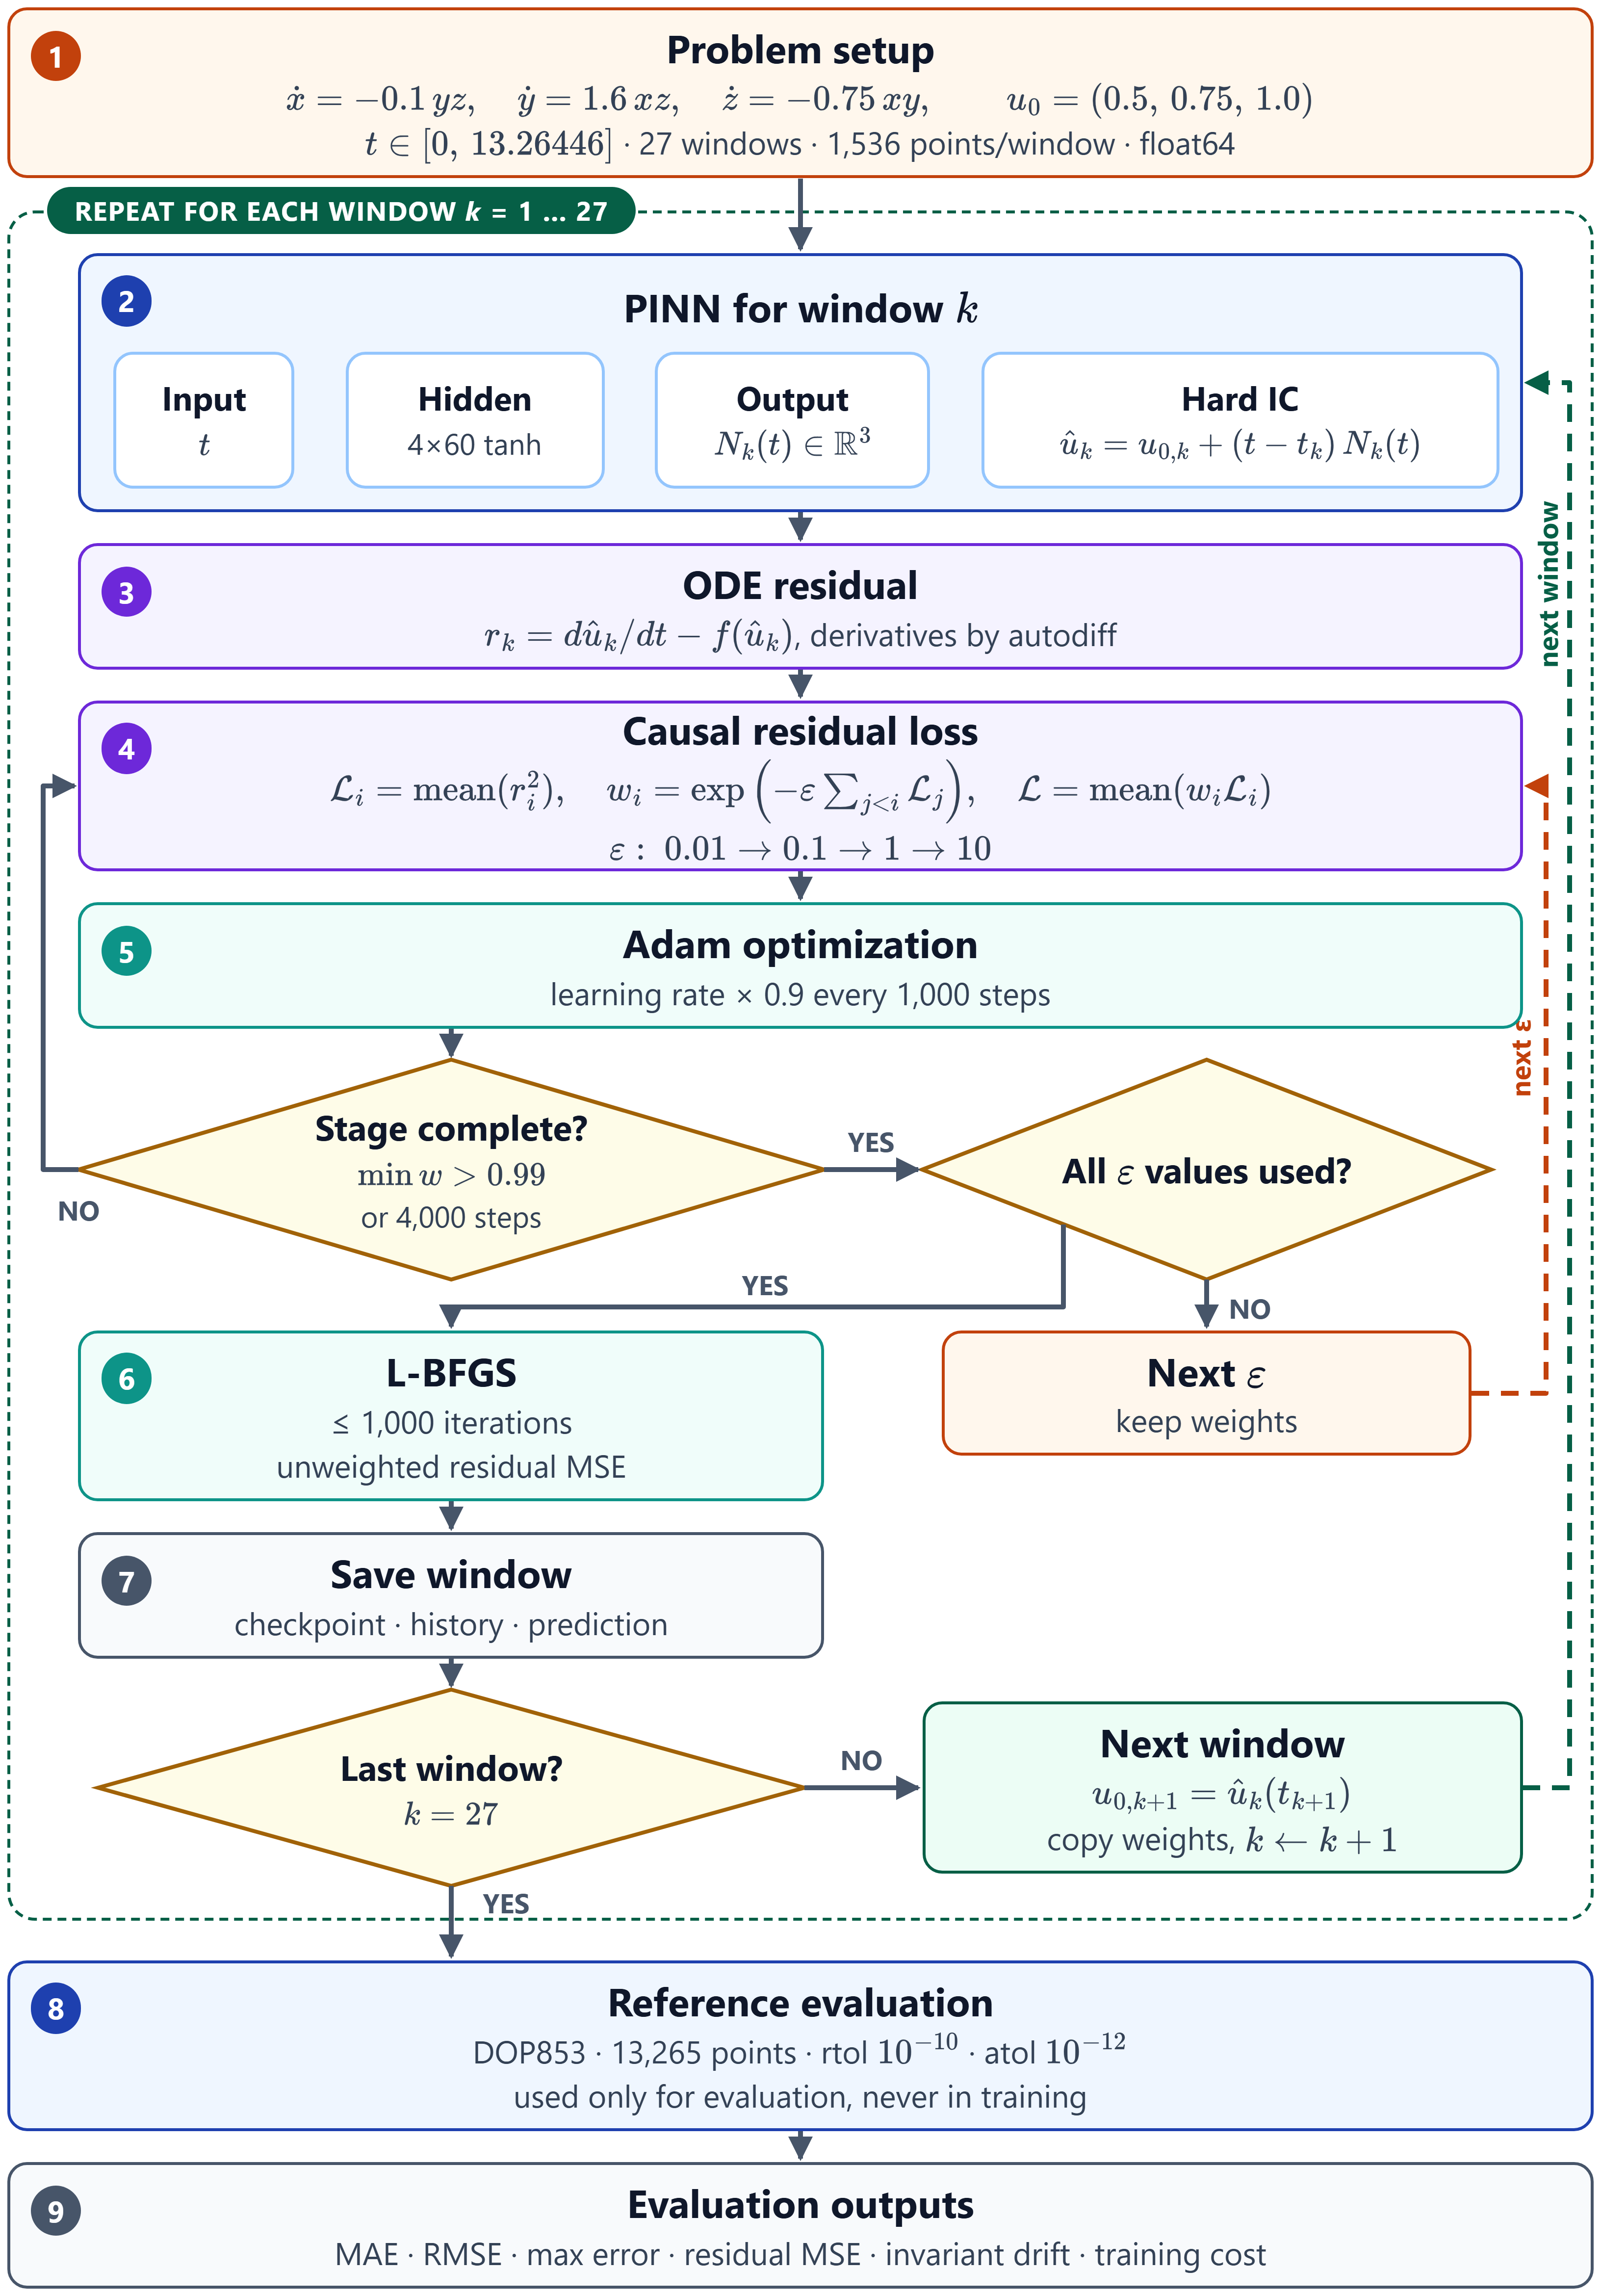
\includegraphics[width=\columnwidth]{figures/method.png}
\caption{Complete implementation pipeline}
\label{fig:pipeline}
\end{figure}

\subsection{Training Loss}
To predict and train the networks of each window, we split the time range into 1536 uniform collocation points per window. 

\[
\begin{aligned}
n_k&=1536,\qquad i=1,\ldots,n_k,\\
t_{k,i}&=t_k+\frac{i-1}{n_k-1}(t_{k+1}-t_k),\\
n_{\mathrm{unique}}&=27(1536-1)+1=41{,}446,\\
n_{\mathrm{window\ uses}}&=27\cdot1536=41{,}472.
\end{aligned}
\]


Ideally 1535 points for each window and 1 handoff point that becomes the initial state for the next window. While training, all the points in a single window are passed to the network at once which gives an output of shape $(1536,3)$.
Then we apply the trial solution to enforce the intial value. While calculating ODE residuals, pytorch automatic differentiation uses the vectors of x,y,z and create a graph that is differentiable. Pytorch autograd function gives the rate of change for all the collocation points with respect to time. And we use this value and the mathematical derivative to calculate the ODE residual.


\[
\frac{d\hat{u}_k}{dt}
=N_k+(t-t_k)\frac{\partial N_k}{\partial t}.
\]
% PyTorch autograd computes d\hat{u}_k/dt.
% f(\hat{u}_k) evaluates the prescribed ODE vector field.


\begin{equation}
r_k(t)
=\frac{d\hat{u}_k(t)}{dt}
 -f\bigl(\hat{u}_k(t)\bigr)
\in\mathbb{R}^{3}.
\label{eq:residual}
\end{equation}
\[
\begin{aligned}
r_{k,x}(t)
  &=\frac{d\hat{x}_k}{dt}
    +0.1\,\hat{y}_k\hat{z}_k,\\
r_{k,y}(t)
  &=\frac{d\hat{y}_k}{dt}
    -1.6\,\hat{x}_k\hat{z}_k,\\
r_{k,z}(t)
  &=\frac{d\hat{z}_k}{dt}
    +0.75\,\hat{x}_k\hat{y}_k.
\end{aligned}
\]


\[
\mathbf{t}_k
=[t_{k,1},\ldots,t_{k,n_k}]^\mathsf{T}
\in\mathbb{R}^{n_k\times1}.
\]
\[
\mathbf{N}_k,\hat{\mathbf{U}}_k,\dot{\hat{\mathbf{U}}}_k,
\mathbf{F}_k,\mathbf{R}_k\in\mathbb{R}^{n_k\times3}.
\]
% Row i:
% \mathbf{N}_k: N_k(t_{k,i};\theta_k)^\mathsf{T}
% \hat{\mathbf{U}}_k: \hat{u}_k(t_{k,i})^\mathsf{T}
% \dot{\hat{\mathbf{U}}}_k: (d\hat{u}_k/dt)(t_{k,i})^\mathsf{T}
% \mathbf{F}_k: f(\hat{u}_k(t_{k,i}))^\mathsf{T}
% \mathbf{R}_k: r_k(t_{k,i})^\mathsf{T}

For each ordered collocation time $t_{k,i}$, we take the mean of the three squared residual components:

\begin{equation}
\begin{aligned}
L_{k,i}
  &=\frac{1}{3}\left\|r_k(t_{k,i})\right\|_2^2\\
  &=\frac{1}{3}\Bigl(
       r_{k,x}(t_{k,i})^2
      +r_{k,y}(t_{k,i})^2\\
  &\hspace{3.8em}+r_{k,z}(t_{k,i})^2
    \Bigr)
  \in\mathbb{R}_{\geq0}.
\end{aligned}
\label{eq:pointloss}
\end{equation}

To solve a long horizon time dependent ODE system, only residual loss is not sufficient. Thats why use we used causal weights and causal weighted loss. The causal weight at a time depends on the accumulated residual loss at earlier times \cite{wang2024causal}:

\[
S_{k,i}=\sum_{j=1}^{i-1}L_{k,j},
\qquad
S_{k,1}=0.
\]
\begin{equation}
w_{k,i}
=\exp\left(-\epsilon S_{k,i}\right)
=\exp\left(-\epsilon\sum_{j=1}^{i-1}L_{k,j}\right).
\label{eq:weights}
\end{equation}
\[
\begin{gathered}
w_{k,1}=1,\qquad 0<w_{k,i}\leq1,\\
\epsilon\in\{0.01,0.1,1,10\}.
\end{gathered}
\]
\begin{equation}
\mathcal{L}_{k,\epsilon}
=\frac{1}{n_k}
 \sum_{i=1}^{n_k}w_{k,i}L_{k,i}
\in\mathbb{R}_{\geq0}.
\label{eq:causalloss}
\end{equation}
\[
\begin{aligned}
\mathbf{L}_k
  &=[L_{k,1},\ldots,L_{k,n_k}]^\mathsf{T}
   \in\mathbb{R}^{n_k},\\
\mathbf{w}_k
  &=[w_{k,1},\ldots,w_{k,n_k}]^\mathsf{T}
   \in\mathbb{R}^{n_k}.
\end{aligned}
\]
% k: window index; i: current point; j: earlier point.
% \epsilon: scalar causal-weighting parameter.
% \mathcal{L}_{k,\epsilon}: one scalar objective at current parameters.
% Weights are recomputed, then detached for gradient calculation.

Here $n_k=1536$. $L_{k,j}$ in \eqref{eq:weights} means the error at earliar points of $i$, where $j < i$ and $L_{k,i}$ means the loss at collocation point $i$ in \eqref{eq:causalloss}. $w_{k,i}$ denotes the causal weights of the collocation points. Here the causal weights are fixed while Adam optimizer calculated the gradient. We used four $\epsilon$ stages: $0.01$, $0.1$, $1$, and $10$  to reduce the earlier points error, and increase the weights. $\epsilon$ in the equation means the penalty for the models in each stages. Model must try to reduce the earlier loss to improve each points weights.

Only using ODE residual isn't enough for long horizon system like Lorenz system. And specially for the windowed algorithm, early times should be fitted before late times, as the errors accumulates and backtracking isn't possible. Therefore, later states depend on the earlier states, if earlier error is reduced, possibly the later error can be reduced as well. To address this, we first calculate the per-collocation point loss, $L_{k,i}$ which is the mean of the three squared ode residuals at time $i$. We assign weights for each point in time. Each points weight updates its value with the accumulated loss of all earlier points. The Causal loss \eqref{eq:causalloss} is the weighted mean of the residual loss. Weights are recomputed at every epoch. Later section explains the stopping rules of the stages and unweighted L-BFGS refinement steps. 

\subsection{Training Procedure}

The causal loss defined in above, is minimized seperately in each window. Figure \ref{fig:pipeline}
summarize the sequence across the windows. Algorithm \ref{alg:training} gives the training steps. In each window a Adam optimizer and StepLR scheduler is created. The rate of the scheduler is $10^{-3}$ and it is multiplied by 0.9 for every 1,000 updates. It is maintained for the four stages of $\epsilon=(0.01,0.1,1,10)$ across the window. There is a 4,000 update limit for each stage. When the saved minimum weight is above 0.99 or if there is an Adam update then the code will recalculate the causal weights at all collocation points at that particular window. If the minimum causal weight from the entire window among 1535 points is above 0.99 then it moves to the next $\epsilon$ stage. If it is below 0.99 and it reaches the epoch threshold then it moves to the next stage and records failure. When all four stages are completed then L-BFGS tries to minimize the loss using unweighted residual mean up to 1,000 epoch. 

\[
\mathcal{L}^{\mathrm{raw}}_k
=\frac{1}{n_k}\sum_i L_{k,i}
=\frac{1}{3n_k}\sum_i\|r_k(t_{k,i})\|_2^2.
\]

To keep track of training we use a snapshot at every 50 epoch to keep training history.

The code saves the parameters of each window, transfers the endpoint state, and copies the parameters to the next trainable window. The config file has the same configuration as all modules were, initial states, training history, next window, PyTorch, NumPy etc. A different configuration in a config is rejected. The run also outputs stage status and residual snapshots. DOP853 values are captured at set up evaluative points. They do not enter the loss, gradient, or stopping test. After training, a dedicated custom function collects all the artifacts and evaluates the final piecewise model and its residual on the collocation and evaluation grids. Finally, a summary function computes error and invariant measures from these arrays. The reported full residual is one of the evaluation.

\begin{algorithm}[t]
\caption{Sequential causal window training}
\label{alg:training}
\begin{algorithmic}[1]
\Require Ordered windows $W_0,\ldots,W_{26}$ and their uniform time points
\State Set $u_{0,0}\gets[0.5,0.75,1.0]^\mathsf{T}$
\For{$k=0,\ldots,26$}
  \If{$k>0$}
    \State Set $u_{0,k}\gets\hat{u}_{k-1}(t_k)$
    \State Initialize $\theta_k\gets\theta_{k-1}$
  \EndIf
  \State Add $t_{k+1}$ to the residual points if $k<26$
  \For{$\epsilon\in(0.01,0.1,1,10)$}
    \For{at most 4,000 Adam steps}
      \State Use ordered times $t_{k,i}$, $i=1,\ldots,n_k$
    \State Evaluate $N_k(t_{k,i};\theta_k)\in\mathbb{R}^{3}$
    \State Form $\hat{u}_k(t_{k,i})$ using \eqref{eq:trial}
    \State Compute $d\hat{u}_k/dt$ by automatic differentiation
    \State Evaluate $f(\hat{u}_k)$ and form $r_k$ using \eqref{eq:residual}
    \State Compute $L_{k,i}$ using \eqref{eq:pointloss}
    \State Compute $w_{k,i}$ using \eqref{eq:weights}; detach weights
      \State Backpropagate \eqref{eq:causalloss}; Adam then StepLR
      \If{verified post-update $\min_i w_{k,i}>0.99$}
        \State \textbf{break}
      \EndIf
    \EndFor
    \State Record whether the threshold was met or capped
  \EndFor
  \State Run L-BFGS on the unweighted residual loss
  \State Save window model, endpoint state, and config record
\EndFor
\end{algorithmic}
\end{algorithm}

\section{Experimental Setup}
This section explain the experimental setup for the saved windowed run. It contains the configuration and reference information, the evaluation measures and the separate full interval comparison.




\subsection{Reference Solution}




Table \ref{tab:config} shows the parameters used for the reported windowed run. We use SciPy’s DOP853 \cite{virtanen2020} as the numerical reference, a relative tolerance of $10^{-10}$ and a absolute tolerance of $10^{-12}$. It is sampled at 13,265 equally-spaced time points, and Distances away from training grid. This is a numerical reference at specified tolerances.


\begin{table}[t]
\caption{windowed-run configuration}
\label{tab:config}
\centering\footnotesize
\begin{tabular}{ll}
\toprule
Setting & Value\\
\midrule
Interval; windows & $[0,13.26446]$; 27 equal windows\\
Network per window & $1$--$60$--$60$--$60$--$60$--$3$, tanh\\
Parameters & 11,283 per window\\
Initial condition; precision & 0.5, 0.75, 1.0; float64\\
Uniform collocation grid & 41,446 unique points\\
Adam $\epsilon$ stages & $0.01,0.1,1,10$\\
Stage threshold; epoch limit & min$\_w_{k,i}>0.99$; 4,000\\
Adam rate; scheduler & $10^{-3}$; $\times0.9$ per 1,000 steps\\
L-BFGS budget & at most 1,000 iterations/window\\
Warm start; seed & Initialize $\theta_k\gets\theta_{k-1}$; 0\\
Reference grid & 13,265 uniform times\\
\bottomrule
\end{tabular}
\end{table}

\subsection{Evaluation}
\[
\begin{aligned}
e(t_j)&=\hat{u}(t_j)-u_{\mathrm{ref}}(t_j)\\
&=[e_x(t_j),e_y(t_j),e_z(t_j)]^\mathsf{T}\in\mathbb{R}^{3},\\
&\qquad j=1,\ldots,n_{\mathrm{eval}}.
\end{aligned}
\]
\begin{equation}
\begin{aligned}
\operatorname{RMSE}_2
  &=\left(
      \frac{1}{n_{\mathrm{eval}}}
      \sum_{j=1}^{n_{\mathrm{eval}}}
      \|e(t_j)\|_2^2
     \right)^{1/2}\\
  &=\left(
      \operatorname{RMSE}_x^2
     +\operatorname{RMSE}_y^2
     +\operatorname{RMSE}_z^2
     \right)^{1/2}.
\end{aligned}
\label{eq:rmse}
\end{equation}

\[
\begin{aligned}
\operatorname{MAE}_c&=\frac{1}{n_{\mathrm{eval}}}\sum_j|e_c(t_j)|,\\
\operatorname{RMSE}_c&=\left(\frac{1}{n_{\mathrm{eval}}}\sum_j e_c(t_j)^2\right)^{1/2},\\
\operatorname{Max}_c&=\max_j|e_c(t_j)|,\quad c\in\{x,y,z\},\\
E_{\mathrm{mean}}&=\frac{1}{n_{\mathrm{eval}}}\sum_j\|e(t_j)\|_2,\\
E_{\mathrm{max}}&=\max_j\|e(t_j)\|_2.
\end{aligned}
\]



while the combined maximum error is $\max_j\|e(t_j)\|_2$. 
The dense-grid residual mean square is the average of the three residual components squared, taken over the times of the evaluation. The comparison run is with the same network depth and width for the entire interval [0, T]. The windowed run simultaneously changes the number of networks, the grid, loss, warm start and
the optimizer schedule. We measuere their final output and compare them.






\section{Results}
This section reports the measurements taken from the completed training artifacts. We first look at what the windowed model does correctly and how well it follows the true path and physics. We then compare these results with the baseline reference and a single-network run for comparison with the behaviour of the model.

\subsection{Prediction Accuracy}
We compare the windowed PINN with an extremely accurate numerical reference which is SciPy's DOP853. As shown in Table \ref{tab:errors}, our model achieved a combined RMSE of $6.97\times10^{-5}$ across the 13,265 uniform times in our evaluation grid. The highest state error norm was $3.09\times10^{-4}$. Figure \ref{fig:trajectory} plots these predictions against the reference over time. The trajectories are shown to overlap completely but the error show small peaks in the errors particularly at $t\simeq5$.

\begin{table}[t]
\caption{Windowed-run error against DOP853 on 13,265 times}
\label{tab:errors}
\centering\footnotesize
\begin{tabular}{lccc}
\toprule
State & MAE & RMSE & Maximum\\
\midrule
$x$ & $1.89\times10^{-5}$ & $2.74\times10^{-5}$ & $1.13\times10^{-4}$\\
$y$ & $2.94\times10^{-5}$ & $4.96\times10^{-5}$ & $2.88\times10^{-4}$\\
$z$ & $2.78\times10^{-5}$ & $4.05\times10^{-5}$ & $1.30\times10^{-4}$\\
State norm & $5.12\times10^{-5}$ & $6.97\times10^{-5}$ & $3.09\times10^{-4}$\\
\bottomrule
\end{tabular}
\end{table}

\begin{figure}[t]
\centering
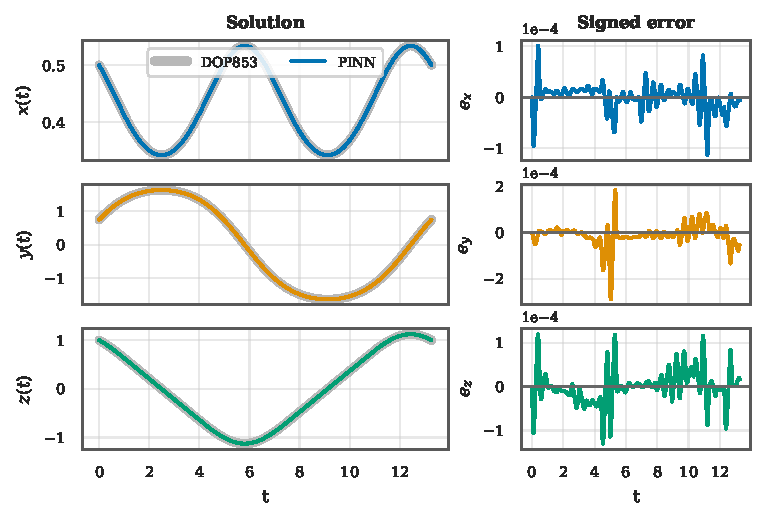
\includegraphics[width=\columnwidth]{figures/solution_vs_reference.pdf}
\caption{PINN solution vs reference with signed errors.}
\label{fig:trajectory}
\end{figure}

We also measured how closely the model obeyed the underlying equations. The MSE of the ODE residual was very small on the evaluation grid at $1.872\times10^{-7}$. Also the residual MSE of windowed run on collocation grid is nearly same ($1.874\times10^{-7}$). The DOP853 reference drifted less than $4\times10^{-10}$ for perspective.

Lastly, the hard trial solution ensures that the values of the state are exactly continuous at the inner 26 interfaces connecting the windows.


\subsection{Run Comparison}
The differences with respect to the two saved configurations are shown in Table \ref{tab:comparison}. The RMSE value of the entire interval network is 2.237, which is much larger than the windowed run network's RMSE value of $6.97\times10^{-5}$. It is a notable result for the recorded settings of this initial value problem. All of the above are uncontrolled types of ablation in the concept of causal weighting \cite{wang2024causal}, windowing \cite{penwarden2023} and warm starts as well as precision and even L-BFGS. In particular the model with the window is much more complicated with 27 times as many parameters and a different collocation grid. Reducing the parameter count of each network might result in similar error.

\begin{table}[t]
\caption{Saved full-interval and windowed runs on the same IVP}
\label{tab:comparison}
\centering\footnotesize
\begin{tabular}{lcc}
\toprule
Measure & One network & 27 windows\\
\midrule
Trainable parameters & 11,283 & 304,641\\
Training points & 39,793 LHS & 41,446 uniform\\
Combined state RMSE & 2.237 & $6.97\times10^{-5}$\\
Maximum state-error norm & 3.346 & $3.09\times10^{-4}$\\
Collocation residual MSE & $2.80\times10^{-4}$ & $1.87\times10^{-7}$\\
Recorded wall time (s) & 4,529 & 881\\
\bottomrule
\end{tabular}
\end{table}

The 27 run windows had 34,765 Adam updates and 1000 L-BFGS closure evaluations per window. Closure evaluations are function calls made by L-BFGS, not iterations. Only two of the 108 causal stages ended at the 4,000-step cap without meeting the $0.99$ weight threshold.
\section{Discussion and Limitations}
There are a few limitations of our method. The trial solution \cite{lagaris1998} defines the initial state for each window exactly. The values remain continuous at the boundaries, but the derivatives can still change suddenly at the boundaries. This comparison with the single network is only a description of two saved runs. The two runs differed in a number of things, including the number of networks, grid, loss and schedule. There was not a windowed run that was saved without using causal weights, because \cite{wang2024causal} they are finding was respecting causality gives one or two order less error. This research applies to only one seed, one initial state and one coefficient set. Other initial states and other coefficient sets may result in different behavior. There is a weakness with the handoff. All windows that follow the first window begin from a predicted state and not the actual state. This means that errors from earlier windows get carried over to later windows. Only 2 of the 108 causal stages were at the 4,000-step limit but failed to reach the $0.99$ weight limit. The causal weights Wang \emph{et al.} vary depending on the number and spacing of the collocation points so if we increase the number of collocation points that will decrease the training loss. To obtain a fairer future test, one and only one training option will be changed at a time, with several seeds.

\section{Conclusion}



Each of our 27 window PINN passes each of the tests on the nearly closed Lorenz-system interval $[0,13.26446]$. The next window was predicted to be at the end. The saved run had a combined state RMSE of $6.97\times10^{-5}$ in comparison to DOP853. A network designed separately to full intervals recorded an RMSE of 2.237. Future research will focus on matched configurations and initial states and generalise to problems with specified boundary conditions at each end.








\bibliographystyle{IEEEtran}
\bibliography{references}

\end{document}
